\chapter{Modélisation du convertisseur CC-CC}
\section{Fonctionnement d'un onduleur monophasé à 2 niveaux}
L'onduleur monophasé à 2 niveaux est composé de deux IGBT. Ils correspondent à un bras d'onduleur, tel que présenté à la figure \ref{circuit_AFE_2L_RC}. Soit une charge $RL$ théorique, dont la résistance se nomme $R$ et l'inductance $L$, on constate que si l'on applique un échelon de tension à la grille de l'IGBT supérieur et que l'on considère l'IGBT comme étant sans pertes et que l'on suppose qu'il entre en saturation avec un échelon unitaire, l'équation de circuit se résume à celle présentée à l'équation \ref{eq1}. À noter que l'échelon unitaire est défini comme: $u(t<0) = 0, u(t\geq 0) = 1)$.

\begin{equation}
\label{eq1}
v(t) = R i(t) + L \frac{d i(t)}{dt}
\end{equation}

On considère que les diodes branchées en parallèle avec les IGBT servent à assurer la continuité du courant lors des commutations.Si l'on néglige la chute de tension aux bornes des IGBT et des diodes, il est possible d'exprimer le courant en fonction de la tension:

\begin{eqnarray}
v(t) &=& V_{DC} u(t)\\
i(t) &=& \frac{V_{DC}}{R} + K \mbox{e}^{\frac{-R}{L}t}\\
i(t=0) &=& i_0\\
K &=& i_0 - \frac{V_{DC}}{R} \\
i(t) &=& i_0  + \frac{V_{DC}}{R}\left(1 - \mbox{e}^{\frac{-R}{L}t}\right)u(t)
\end{eqnarray}

Si l'on définit le temps total d'une modulation par $T$, le temps de conduction de l'alternance positive par $t_{on}$ et le temps de conduction de l'alternance négative par $t_{off}$ il est possible de définir le rapport de modulation $m = \frac{t_{on}}{T} = \frac{1-t_{off}}{T}$. Supposons un rapport de modulation $m_x$, il est possible, si l'on considère le courant initial nul, d'exprimer le courant dans la charge RL pour une période de modulation étant égale à $T$. L'évolution du courant pour une tension appliquée pendant un cycle de modulation est présenté à la figure \ref{eq1}
\begin{figure}
\centering
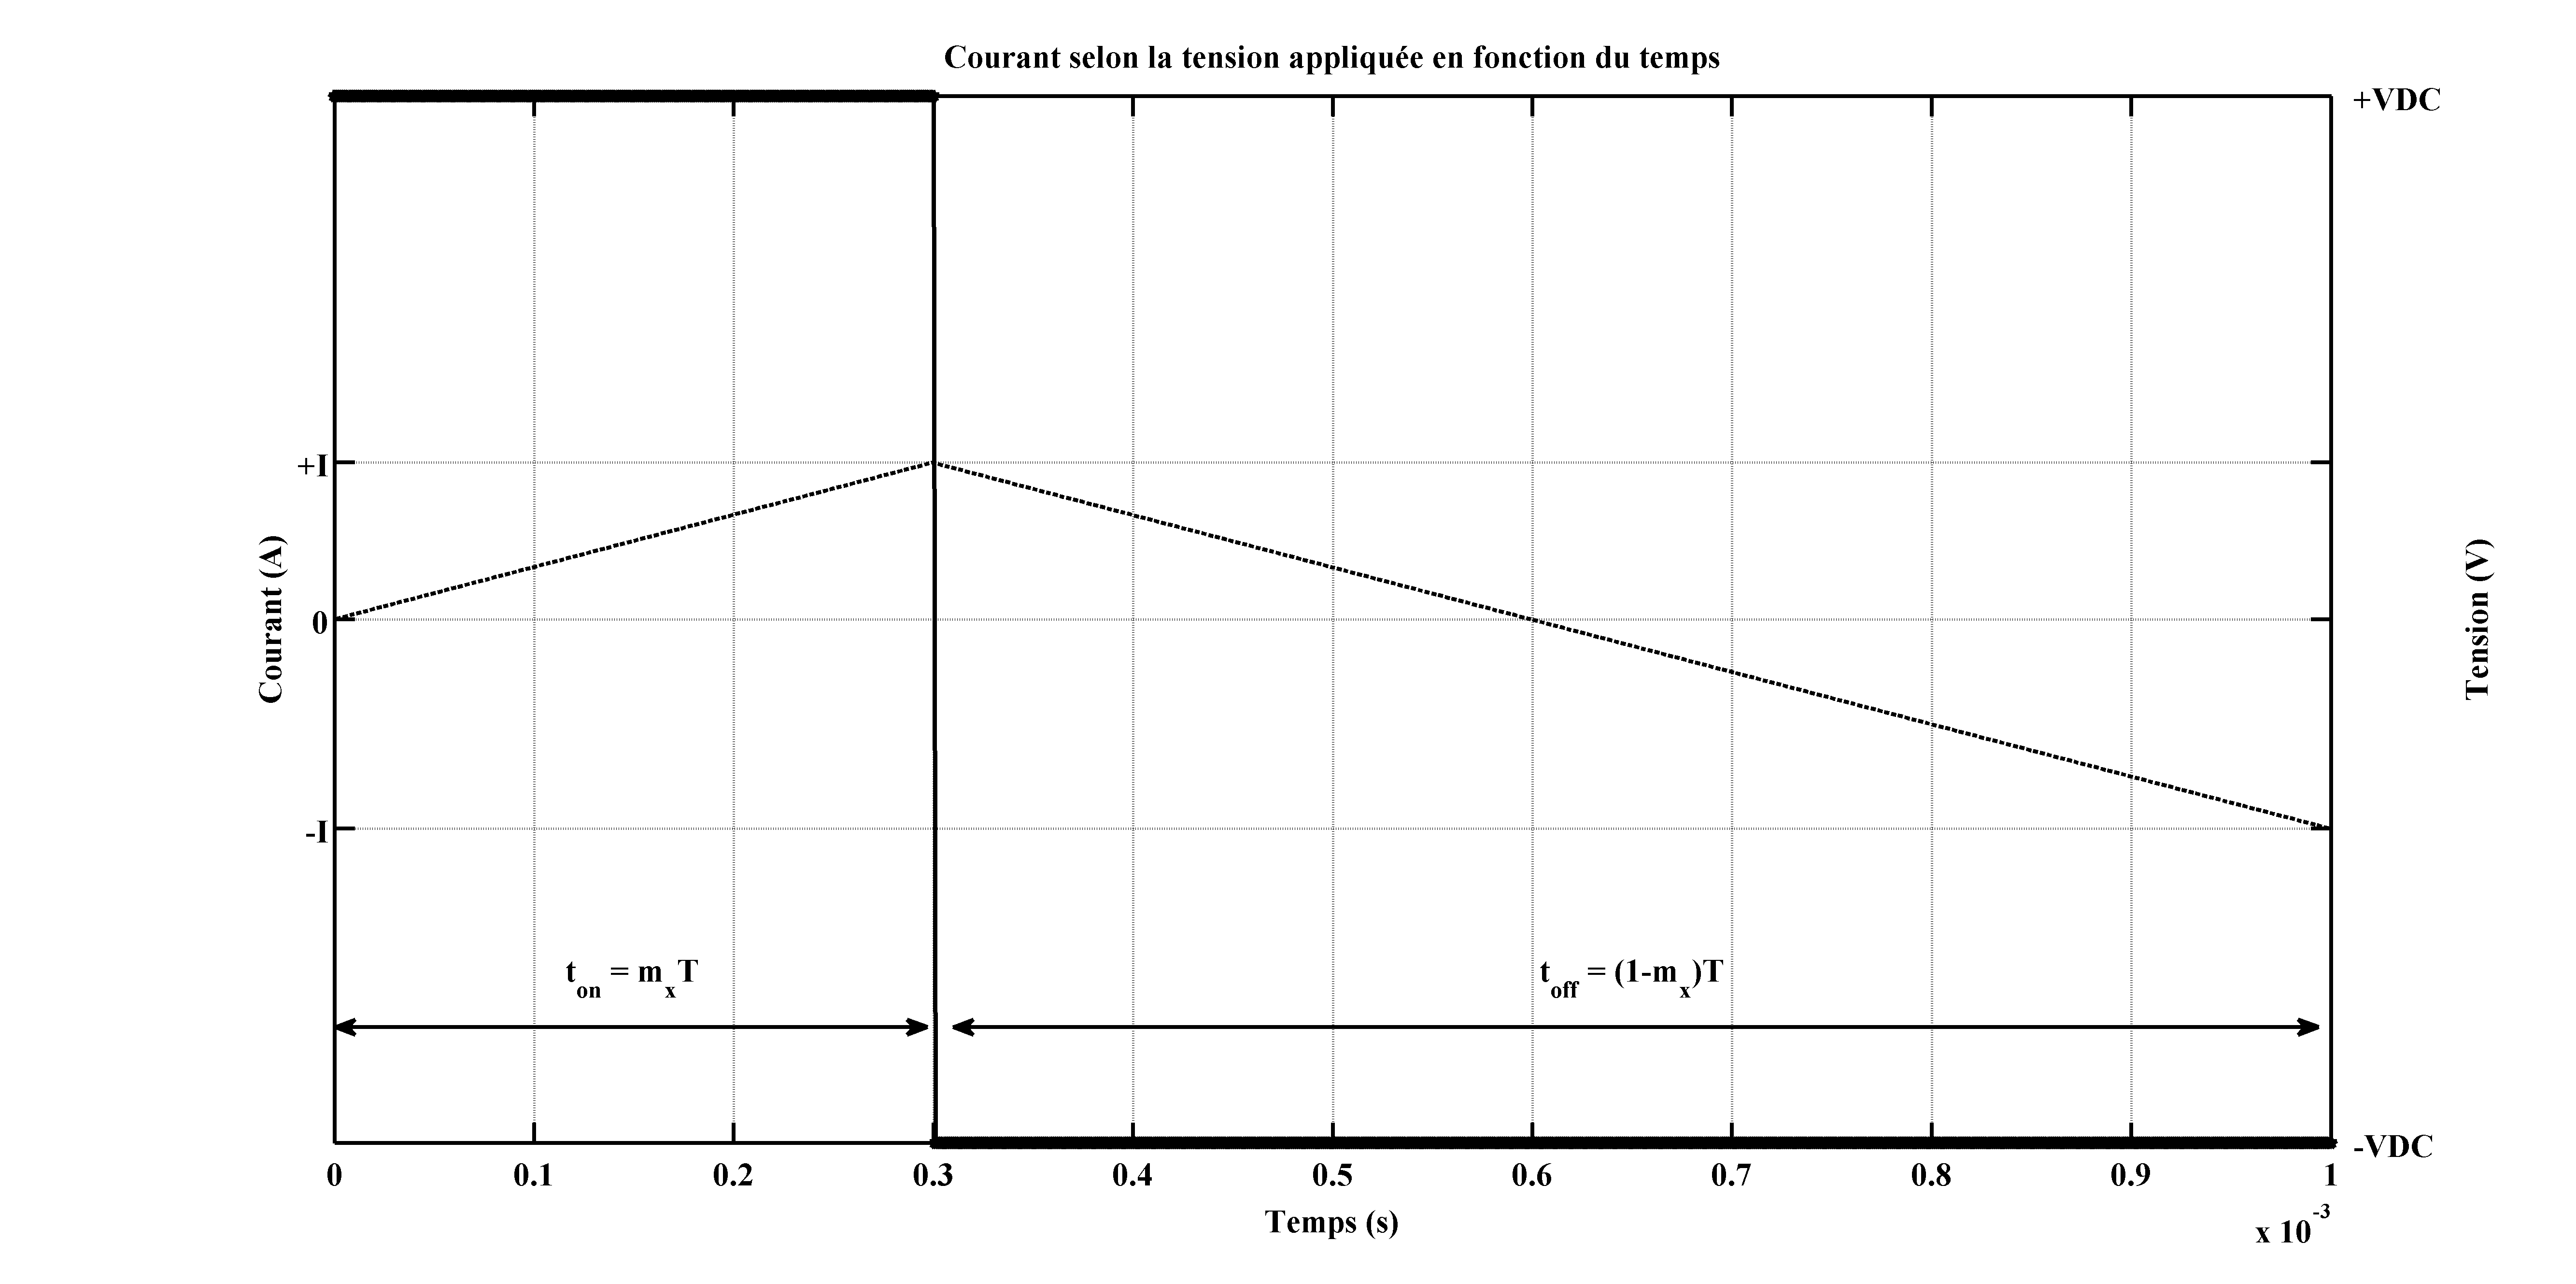
\includegraphics[scale=0.4]{fig/fig_courant_tension_mod.png}
\caption{Courant dans la charge selon une tension $+V_{DC}$ appliquée pendant un temps $t_{on}$ et une tension $-V_{DC}$ appliquée pendant un temps $t_{off}$ pour un cycle de modulation.}
\end{figure}
\begin{eqnarray}
t_{on} &=& m_x T, i_0 = 0\\
i\left(t = t_{on}\right) &=& \frac{V_{DC}}{R}\left(1 - \mbox{e}^{\frac{-R}{L}m_x T}\right)\\
i\left(t = T\right) &=& i\left(t = t_{on}\right) -  \frac{V_{DC}}{R}\left(1 - \mbox{e}^{\frac{-R}{L}(1-m_x)T}\right)
\end{eqnarray}

Afin de faciliter les calculs, on peut approximer $i(t)$ comme une droite de pente constante. On en déduit que $i(t) = \frac{V_{DC}}{L}t$, pour $0\leq t \leq m_x T$ et $i(t) = \frac{V_{DC}}{L} m_x T \left( 2 - t\right)$, pour $m_x\leq t \leq T$. La valeur moyenne sur une période se calcule comme suit:

\begin{eqnarray}
I_{moy} &=& \int_0^{t_{on}} i(t) + \int_{t_{on}}^{T} i(t)\\\label{eq_Imoy}
I_{moy} &\approx & \frac{V_{DC}}{LT}\left(\frac{m_x^2 T^2}{2} -(3m_x^2 -4m_x +1)\frac{T^2}{2}\right)
\end{eqnarray}

Par l'analyse des formes d'ondes en traçant le courant moyen en fonction du rapport de modulation, présenté à la figure \ref{eq1}, on remarque que si l'on a un rapport de modulation inférieur à 0.2929, le courant moyen est négatif et que si le rapport de modulation est supérieur à cette valeur, le courant moyen est positif.

\begin{figure}[htb]
\makebox[\textwidth][c]{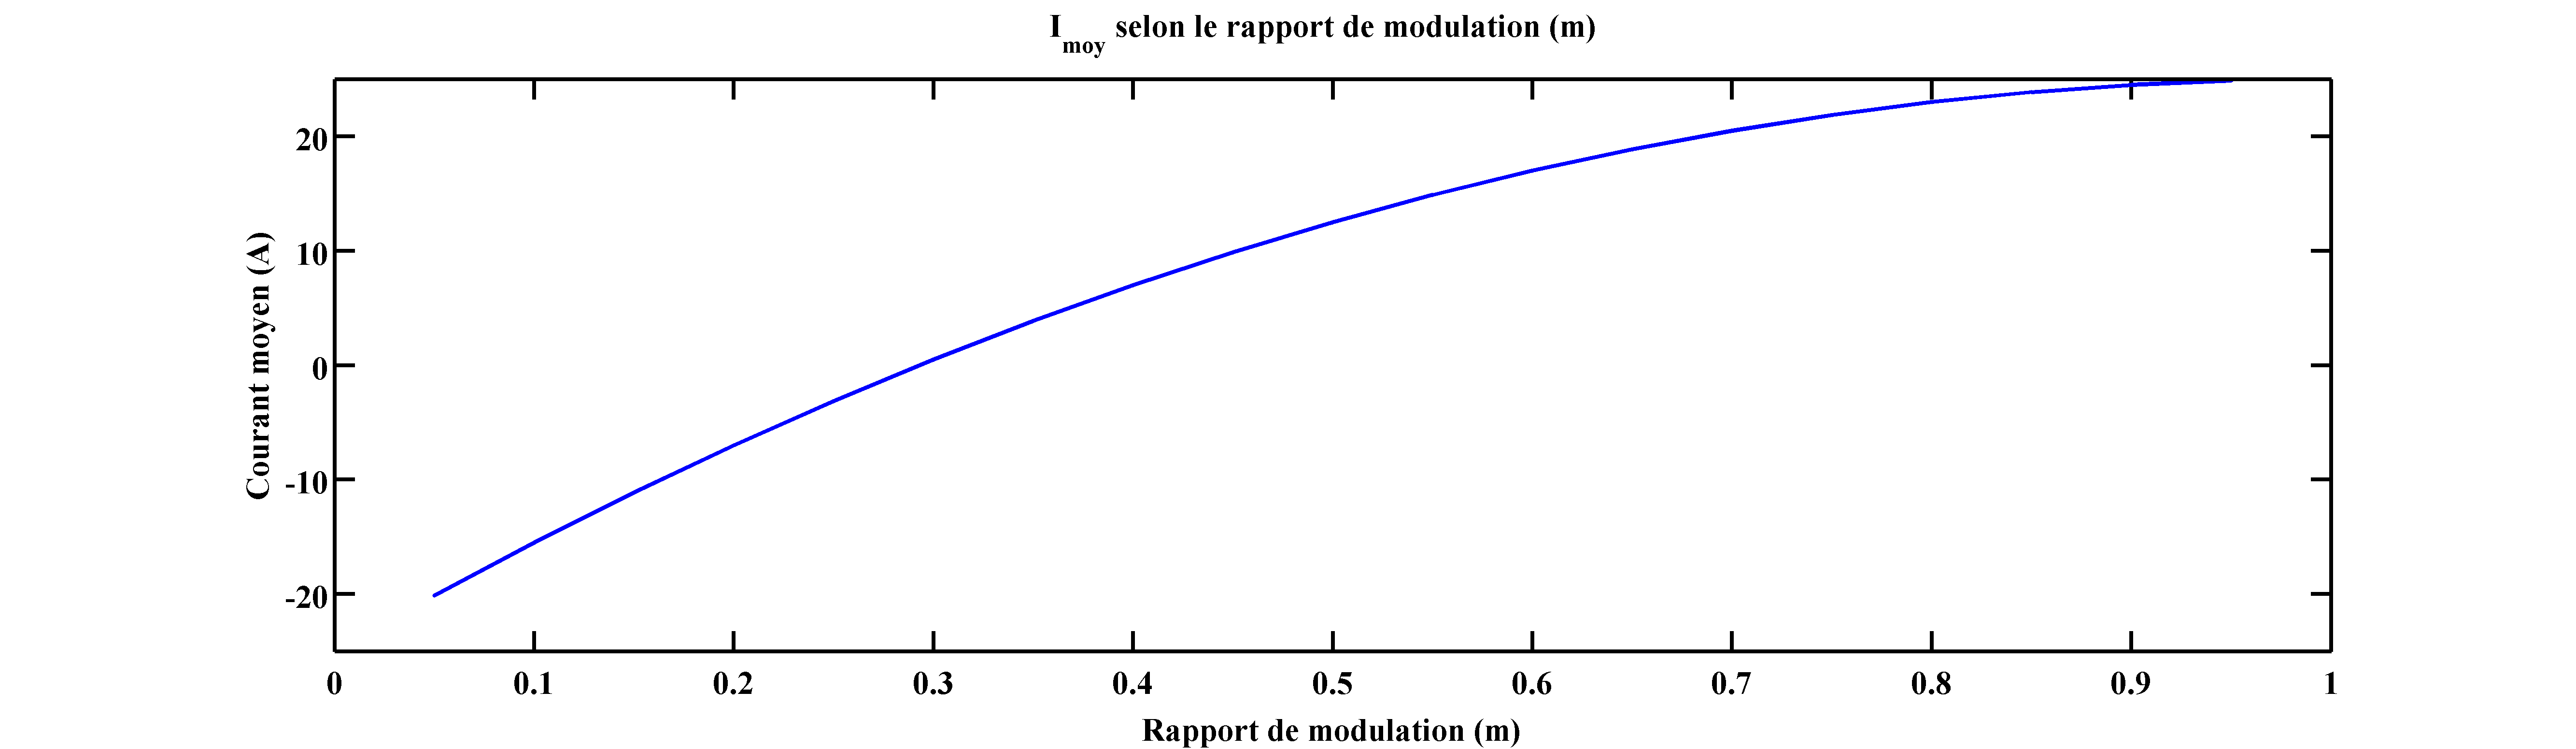
\includegraphics[scale=0.4]{fig/Imoy_m.png}}
\caption{Courant moyen en fonction du rapport de modulation dans un onduleur monophasé}
\end{figure}

\section{Fonctionnement d'un onduleur monophasé NPC à 3 niveaux}
Le schéma d'un onduleur monophasé NPC à 3 niveaux est présenté à la figure \ref{eq1}. Un onduleur monophasé NPC à 3 niveaux est composé de 4 transistors, de 6 diodes et de deux condensateurs rattachés au point neutre (point central sur la figure \ref{eq1}). La configuration présentée a pour objectif d'obtenir des niveaux distincts de tension $V_{DC}$ à appliquer aux bornes des électroaimants. Dans cette configuration, chaque transistor ne commute pas toute la tension $V_{DC}$, l'avantage étant qu'on peut utiliser des composantes dont le dimensionnement est moins imposant que celles nécessaire pour fournir une puissance équivalente dans un montage à 2 niveaux classique. 

\paragraph{}Il existe 4 transistors IGBT qui commutent par paires. Les séquences possibles et les tensions produites sont décrites dans le tableau suivant:

\begin{table}[htb]
\centering
\begin{tabular}{ |c|c|c| }
\hline
  Type de séquence & Transistors activés & Niveau de tension \\\hline\hline
  P & [1,2] & $+V_{DC}$ \\\hline
  N & [3,4] & $-V_{DC}$ \\\hline
  O & [1,3] & $0$ \\\hline
  O & [1,4] & $0$ \\\hline
  O & [2,4] & $0$ \\\hline
\end{tabular}
\end{table}

En excluant les états redondants, il existe 3 états distincts, soit l'état P ([1,2]), l'état N([3,4] et l'état 0([1,3]). Une stratégie de commande simple et applicable est celle d'une modulation MLI à plusieurs niveaux. On réfère ici à la figure \ref{fig_MLI_ML} pour une illustration graphique de la commande MLI multiniveaux. À chaque période de commutation, une comparaison entre l'onde désirée et le signal en dent de scie. Pendant la période où le signal est plus grand (en valeur absolue) que le signal en dent de scie, la paire de transistor associée est activée pendant la période de conduction calculée. 

\begin{figure}[htb]

\makebox[\textwidth][c]{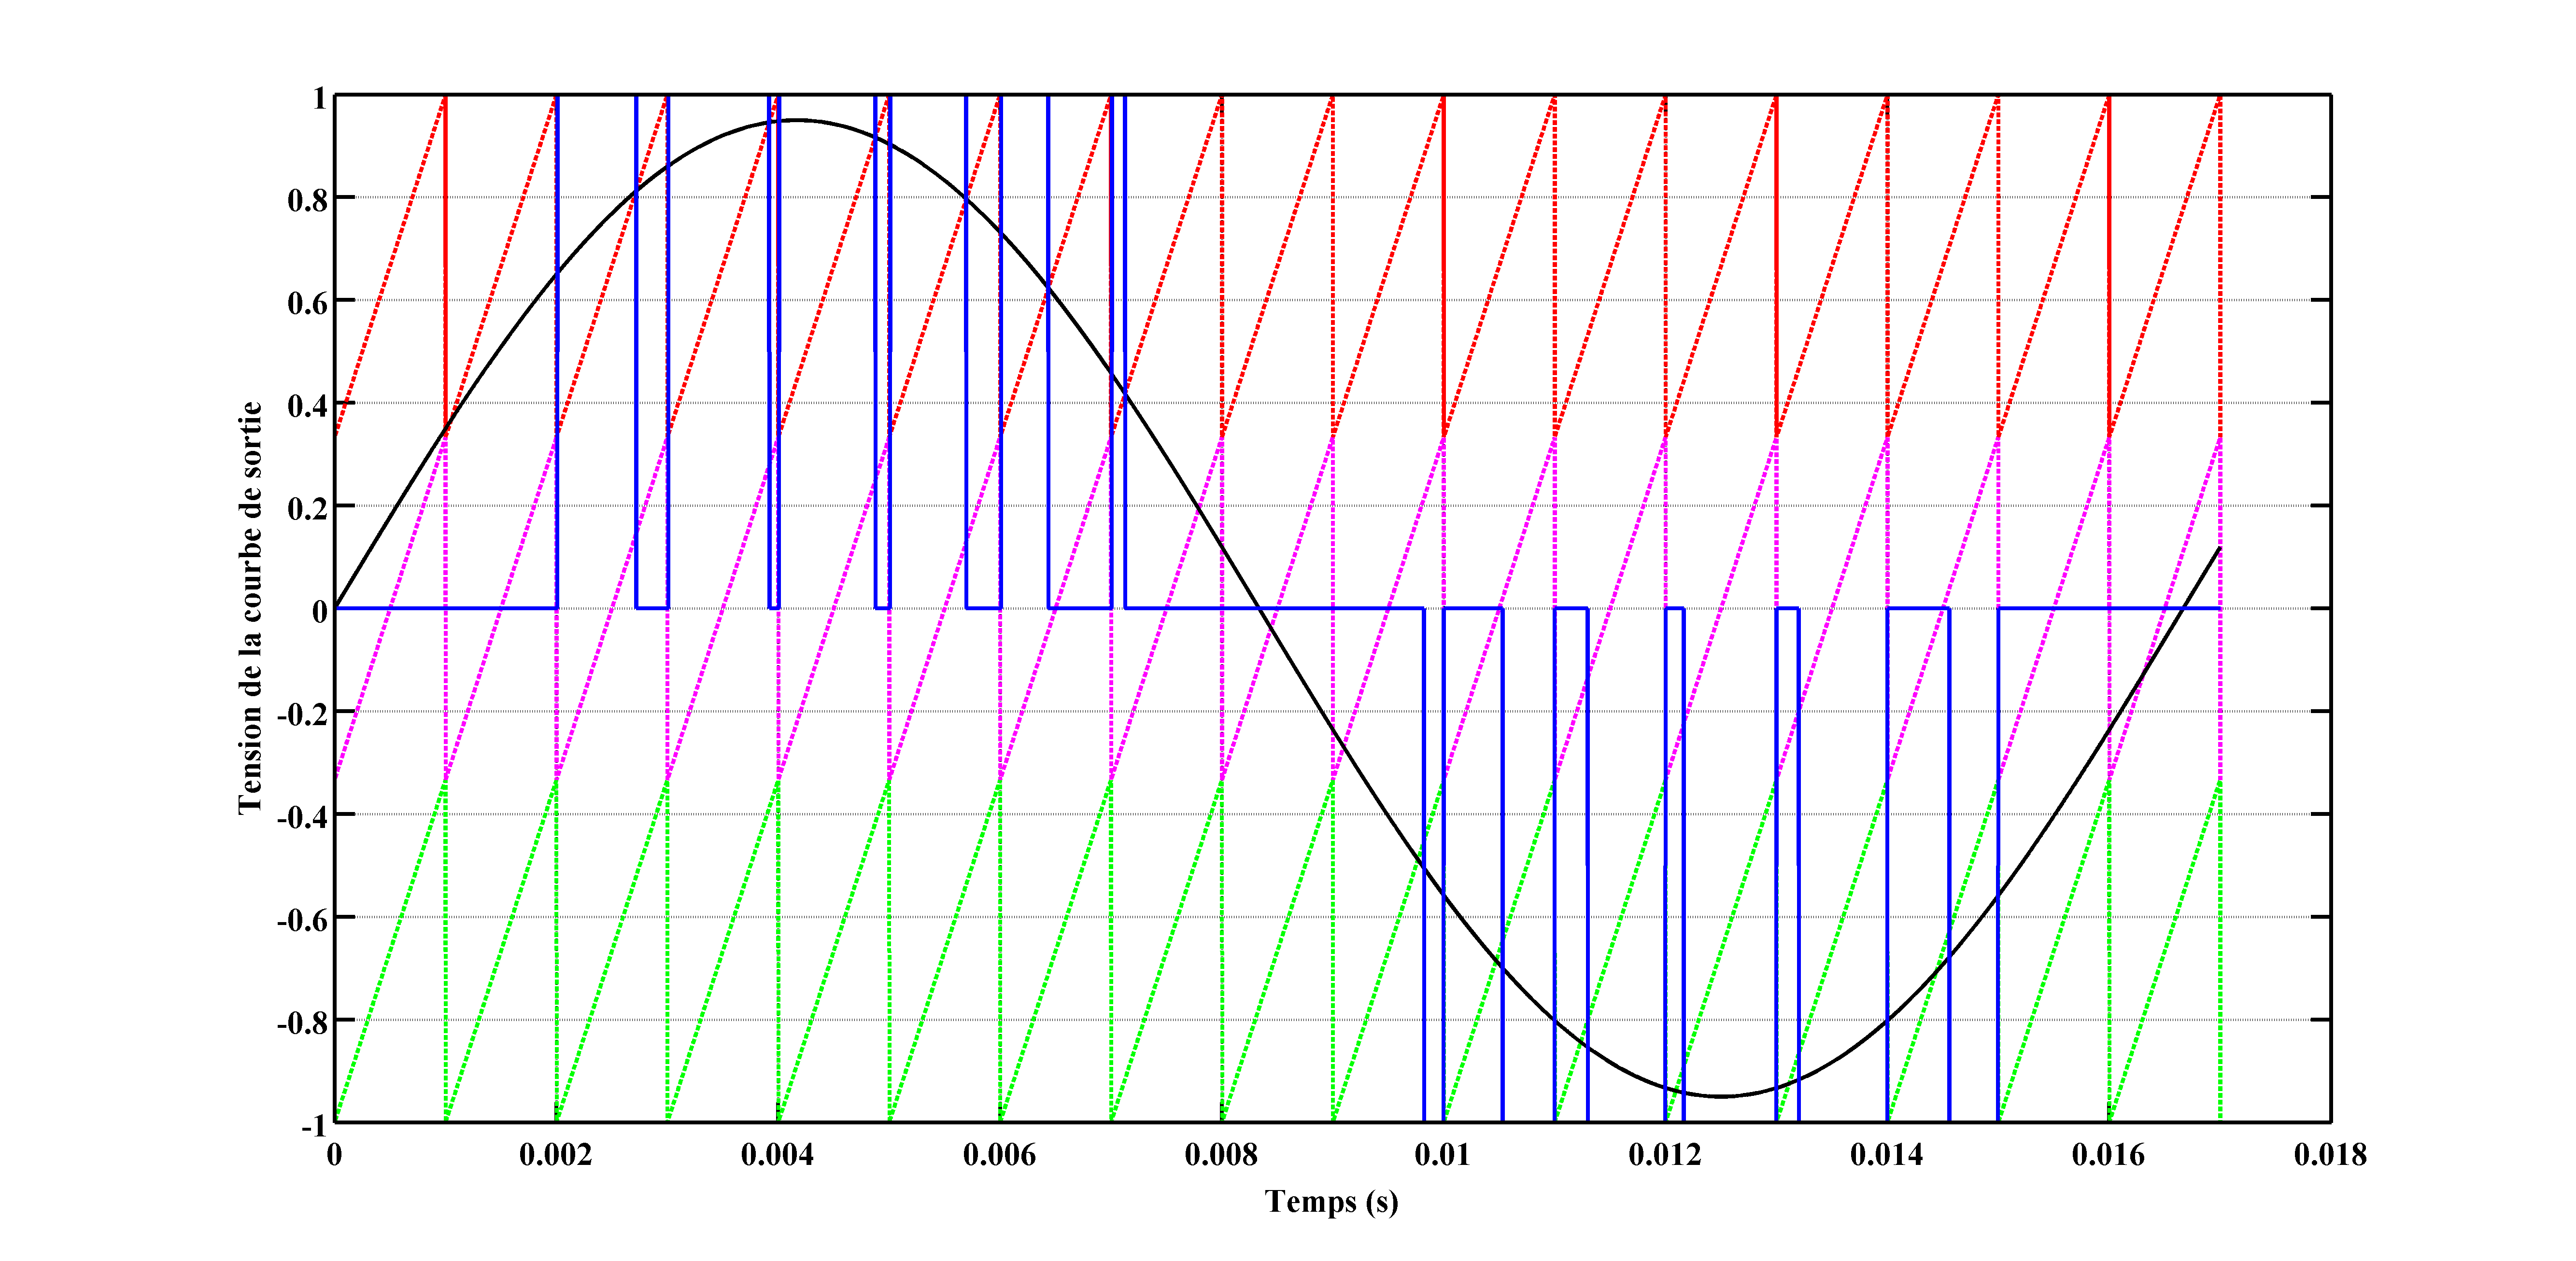
\includegraphics[scale=0.4]{fig/commande_NPC_1.png}}
\caption{Commande MLI multiniveaux pour une consigne sinusoïdale}
\label{fig_MLI_ML}
\end{figure}

\section{Calculs théoriques liés à l'onduleur NPC 3 niveaux}
L'avantage d'une configuration NPC 3 niveaux est la diminution de la tension vue par chaque interrupteur. On considère premièrement que le bus d'alimentation est un bus CC parfait d'une tension de 5kV (selon les spécifications du projet) et qu'il n'y a pas de baisse de tension en fonctionnement normal. Chaque interrupteur est amorcé au tiers de la fréquence vue à la charge, soit à 330Hz, de plus comme l'onduleur proposé par le client utilise un décalage des phases d'un tiers de période, la conduction de chaque bras est donc limitée à 1ms sur 3ms. La tension vue sur l'interrupteur supérieur est limitée à 2.5kV, étant donné la présence d'un point milieu. L'utilisation de 2 cellules NPC 3 niveau permet d'appliquer $\pm$ 5kV aux bornes de la charge. Les interrupteurs doivent donc minimalement tenir une tension de 2.5kV. 

\paragraph{}L'entrelacement des bras et l'utilisation d'une tension suffisamment élevée sur le bus DC permet de limiter le temps de conduction des IGBT et donc, le courant moyen qui y est vu. Le courant maximal demandé par la charge est de 6000A. Afin de calculer le temps d'exposition maximal d'un interrupteur à ce courant, on utilise la tension minimale atteinte par le bus CC. Cette tension est de l'ordre de 3.25kV. Chaque interrupteur voit la moitié de cette tension. soit 1.625kV. La charge étant modélisée comme une inductance pure de 0.1H. En appliquant l'équation \ref{eq_Imoy}, on détermine que le rapport de modulation minimal est de 0.2929, afin de maintenir un courant moyen nul autour d'une consigne, en supposant qu'on ait un courant dans la charge dont la valeur moyenne ait atteint la consigne désirée. La valeur obtenue à partir de cette équation permet de fournir une première itération pour le calcul du courant $RMS$ circulant dans les interrupteurs. En supposant un rapport de modulation de 0.2929, pour une période de 3ms, avec un courant Imax de 6000A, on peut calculer le courant $RMS$ circulant dans l'interrupteur:
\begin{eqnarray}
I_{RMS} &=& \sqrt{\frac{1}{T}\int_0^{m_xT}I_{max}^2 dt}\\
I_{RMS} &=& \sqrt{333\int_0^{878\mu s}6000^2 dt}\\
I_{RMS} &=& 3244.2A RMS
\end{eqnarray}
Selon la commande appliquée, le $m_x$ peut changer étant donné qu'on ne fixe pas nécessairement un courant $I_{moy}$ à 0. Aussi, il est impératif de considérer les pertes qui peuvent faire fluctuer les résultats. Afin de calculer le courant moyen dans la charge, on suppose qu'une période est égale à 2.4s, tel que spécifié dans la documentation du CERN. Afin de simplifier les calculs, on suppose que chaque bras conduit $\frac{1}{3}$ du temps et donc que la période, vue d'un bras, est de 7.2s. Soit la forme de courant présentée à la figure \ref{fig_ref_courant}. Il est possible de calculer la valeur RMS du courant selon l'équation précédemment décrite précédemment. L'intégrale est réalisée au moyen de Matlab. On trouve que le courant RMS moyen d'un interrupteur d'un bras pour un cycle de 2.4s (7.2s vue de l'interrupteur), est de 1107A. 

\begin{figure}[htb]
\makebox[\textwidth][c]{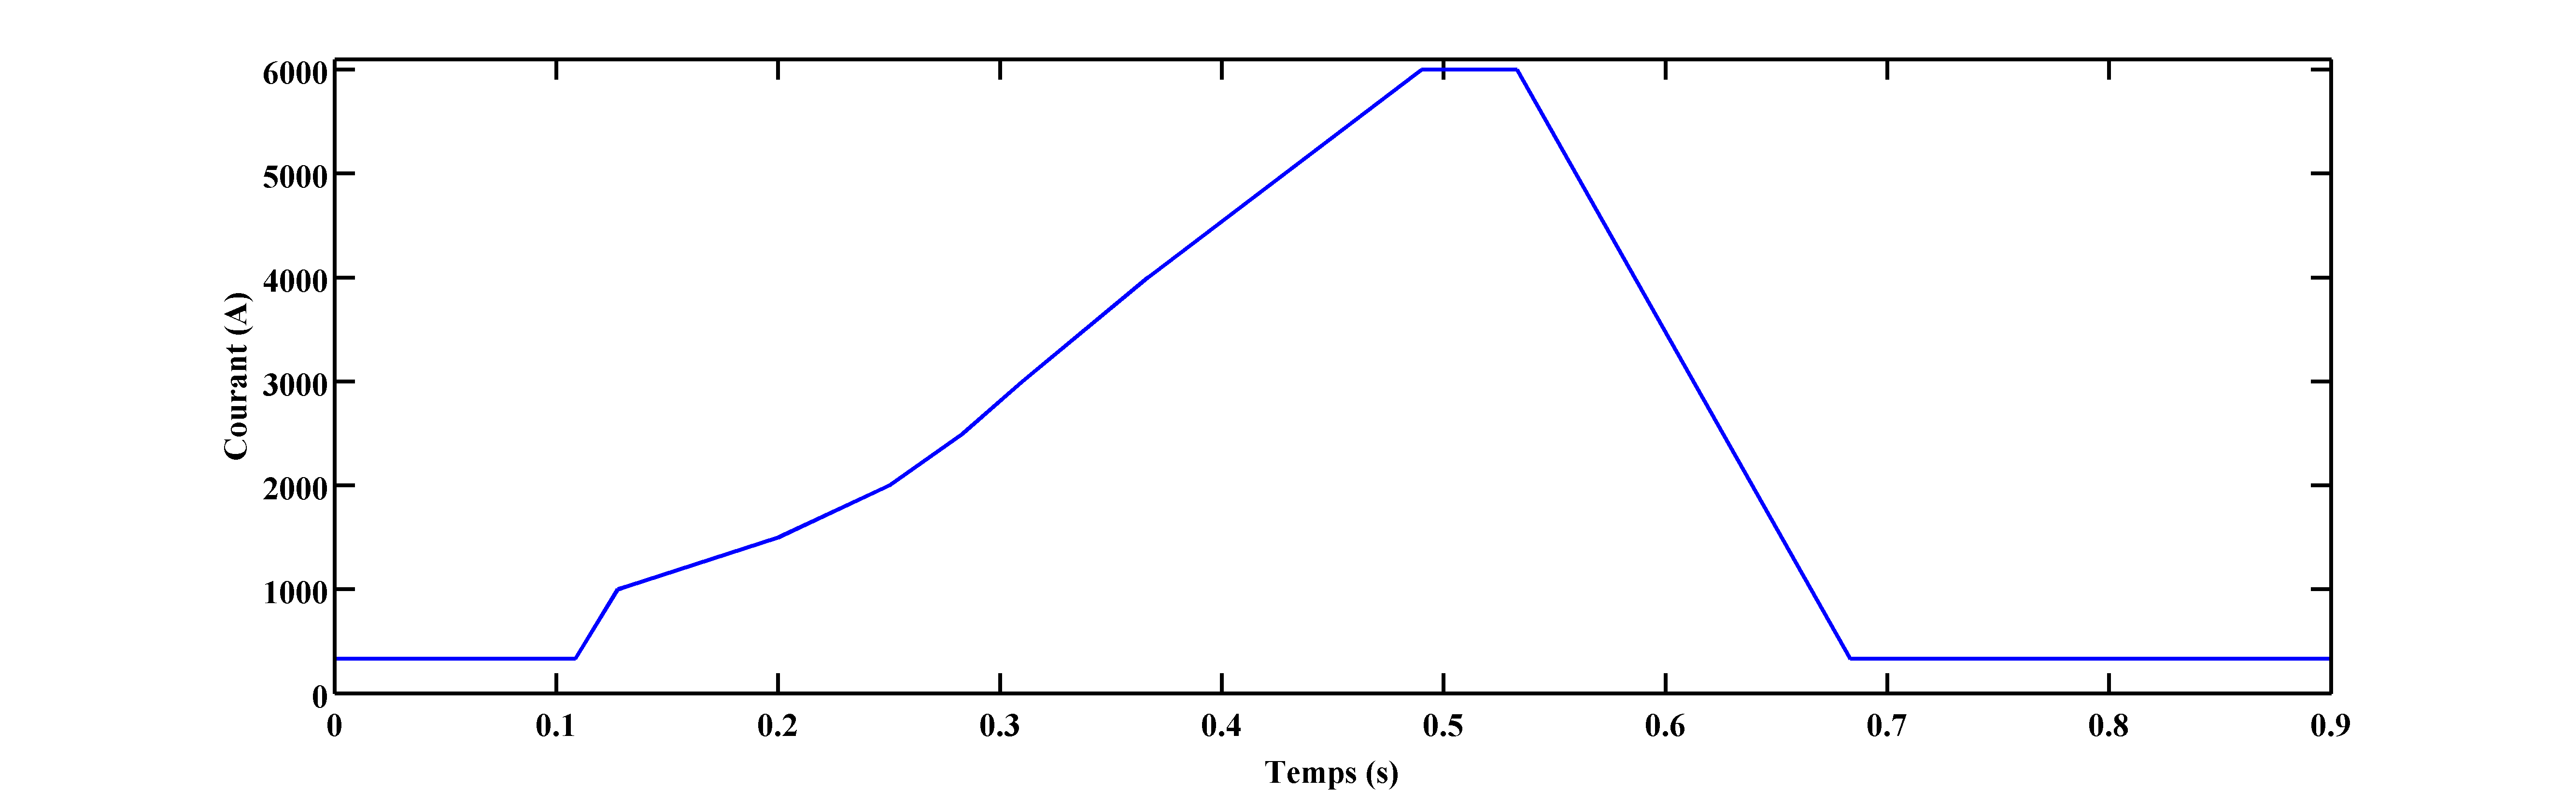
\includegraphics[scale=0.4]{fig/fig_ref_courant.png}}
\caption{Référence de courant des électroaimants en A en fonction du temps (s)}
\label{fig_ref_courant}
\end{figure}

\section{Comparaison des résultats de dimensionnement théoriques obtenus par rapport à ceux du CERN}
Les résultats théoriques et ceux fournis par le CERN sont présentés au tableau \ref{tab_comp_1}. On remarque qu'il est possible d'obtenir un ordre de grandeur respectable des valeurs fournies par le CERN en effectuant des approximations théoriques et en utilisant une version échantillonnée à la main de la courbe de référence de courant. On comprend que les interrupteurs du CERN ne sont pas maintenus à un courant moyen de 0, tel qu'il était prévu, ils sont maintenu à un rapport cyclique (sur 3ms) de 0.25. Ne disposant pas précisément des méhodes de commandes et des formes d'ondes vues à la charge, il est difficile d'obtenir une approximation plus précise. Cependant, on remarque que les interrupteurs sont dimensionnés pour les valeurs RMS maximales vue sur la crête de 6kA et que la valeur moyenne (RMS) des interrupteurs est calculée sur un cycle de 2.4s. L'écart étant faible entre les données calculées théoriquement et celles du CERN, on suppose qu'à cet effet ils utilisent un rapport cyclique de 1/3, soit 1ms/3ms, par interrupteur. La valeur moyenne de tension tient compte que la tension du bus CC peut monter à 5100V. Aussi, si l'on se réfère aux spécifications techniques des interrupteurs employés pour les tests, on remarque que la tension qu'ils tiennent est de l'ordre de 4.5kV. Le courant maximal moyen en valeur RMS varie de 1460 A à 1780 A, selon le type d'interrupteur. La valeur crête du courant RMS respecte les valeurs $I_{MaxComm}$ qui vont de 4000 A à 5500 A.

\begin{table}[htb]
\centering
\begin{tabular}{ |c|c|c| }
\hline
  Paramètre & Théorie & CERN\\\hline\hline
  $I_{FAVRMS}$ (A) & 1107 A & 1070 A \\\hline
  $I_{PeakRMS}$ & 3244 A & 3000 A \\\hline
  $I_{Peak}$ & 6 kA & 6 kA \\\hline
  $V_{AV}$ & 2.5 kV & 2.75 kV \\\hline
\end{tabular}
\caption{Comparatif des résultats théoriques et de ceux fournis par le CERN}
\label{tab_comp_1}
\end{table}